% Generated from Markdown. Edit the .md source, then render again.
\def\solutions{1}
% Editorial and mathematical typesetting rules: templates/attendance-style.md
\PassOptionsToClass{a4paper}{article}
% Find shared files both from the sheet folder (VS Code) and the repo root.
\makeatletter
\def\input@path{{./}{../}}
\makeatother
\documentclass{course_sheet}
\graphicspath{{./}{../}}
\usepackage[T1]{fontenc}
\usepackage{lmodern}
\usepackage{microtype}
\usepackage{needspace}
% Part titles and subsection/exercise numbers are written explicitly.
\setcounter{secnumdepth}{0}
\setlength{\parindent}{0pt}
\setlength{\parskip}{0.2em}
\raggedbottom
\renewcommand{\arraystretch}{1.2}
\usepackage{tikz}
\input{2026-SoSe.tex}
\published{29 September 2026}

% Pandoc emits \tightlist for compact list items; course_sheet.cls does not
% define it (it uses enumitem, not pandoc's convention), so provide it here.
\providecommand{\tightlist}{%
  \setlength{\itemsep}{0pt}\setlength{\parskip}{0pt}}

% \title/\author/\date must be (re)issued after \documentclass so that
% course_sheet.cls's own \maketitle picks up the real sheet title instead of
% its generic "Exercise sheet \sheetname" placeholder.
\title{\\Neural Networks by Hand - Solutions}
\author{}
\date{}

\begin{document}
\maketitle

\Needspace{10\baselineskip}
\section{Part I - A small neural network}

\Needspace{4\baselineskip}
\subsection{Solution 1.1 - Generate the training data}

For $f(x)=-x^2+4x=4-(x-2)^2$, the training data are:

\begin{center}

\begingroup
\setlength{\tabcolsep}{3pt}
\begin{tabular}{@{}p{0.328\linewidth}p{0.638\linewidth}@{}}
\toprule
$x_i$ & $y_i$ \\
\midrule
0 & 0 \\
1 & 3 \\
2 & 4 \\
3 & 3 \\
\bottomrule
\end{tabular}
\endgroup

\end{center}

The parabola has vertex $(2,4)$ and zeros at 0 and 4. At both ends of
the requested interval, $f(-1)=f(5)=-5$.

\begin{center}

\begin{tikzpicture}[x=1.45cm,y=0.48cm]
\draw[->] (-1.2,0)--(5.3,0) node[right] {$x$};
\draw[->] (0,-5.5)--(0,5.2) node[above] {$y$};
\foreach \x in {-1,1,2,3,4,5} {\draw (\x,-0.12)--(\x,0.12);\node[below] at (\x,-0.12) {\small $\x$};}
\foreach \y in {-4,-2,2,4} {\draw (-0.05,\y)--(0.05,\y);\node[left] at (-0.05,\y) {\small $\y$};}
\draw[thin,domain=-1:5,samples=81] plot (\x,{-\x*\x+4*\x});
\foreach \x/\y in {0/0,1/3,2/4,3/3} {\fill (\x,\y) circle (1.6pt);}
\end{tikzpicture}

\end{center}

\Needspace{4\baselineskip}
\subsection{Solution 1.2 - Our neural network architecture}

There are \textbf{seven trainable parameters}: four weights
$w_1,w_2,v_1,v_2$ and three biases $b_1,b_2,c$. The hidden neurons use
ReLU; the output is linear. ReLU is zero for $z\leq0$ and equals $z$ for
$z\geq0$.

\begin{center}

\begin{tikzpicture}[x=0.7cm,y=0.5cm]
\draw[->] (-5.5,0)--(5.5,0) node[right] {$z$};
\draw[->] (0,-0.5)--(0,5.6) node[above] {$\operatorname{ReLU}(z)$};
\draw[thick] (-5,0)--(0,0)--(5,5);
\node[below] at (-5,0) {$-5$};\node[below left] at (0,0) {$0$};\node[below] at (5,0) {$5$};\node[left] at (0,5) {$5$};
\end{tikzpicture}

\end{center}

\begin{center}

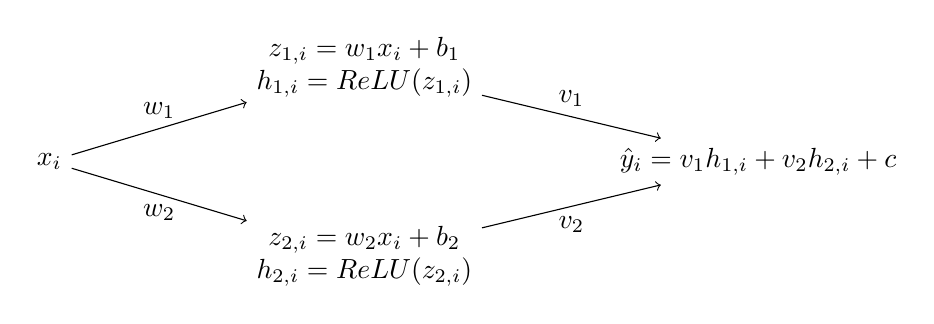
\begin{tikzpicture}[every node/.style={align=center}]
\node (x) at (0,0) {$x_i$};
\node (h1) at (4,1.2) {$z_{1,i}=w_1x_i+b_1$\\$h_{1,i}=\operatorname{ReLU}(z_{1,i})$};
\node (h2) at (4,-1.2) {$z_{2,i}=w_2x_i+b_2$\\$h_{2,i}=\operatorname{ReLU}(z_{2,i})$};
\node (y) at (9,0) {$\hat y_i=v_1h_{1,i}+v_2h_{2,i}+c$};
\draw[->] (x)--node[above] {$w_1$}(h1);\draw[->] (x)--node[below] {$w_2$}(h2);
\draw[->] (h1)--node[above] {$v_1$}(y);\draw[->] (h2)--node[below] {$v_2$}(y);
\end{tikzpicture}

\end{center}

\Needspace{4\baselineskip}
\subsection{Solution 1.3 - A complete forward pass}

With $w_1=1$, $b_1=-0.5$, $w_2=-1$, $b_2=2.5$, $v_1=v_2=1$ and $c=0$,
the hidden-layer values are:

\begin{center}

\begingroup
\setlength{\tabcolsep}{3pt}
\small
\begin{tabular}{@{}p{0.152\linewidth}p{0.152\linewidth}p{0.152\linewidth}p{0.152\linewidth}p{0.152\linewidth}p{0.152\linewidth}@{}}
\toprule
$x_i$ & $y_i$ & $z_{1,i}$ & $h_{1,i}$ & $z_{2,i}$ & $h_{2,i}$ \\
\midrule
0 & 0 & -0.5 & 0 & 2.5 & 2.5 \\
1 & 3 & 0.5 & 0.5 & 1.5 & 1.5 \\
2 & 4 & 1.5 & 1.5 & 0.5 & 0.5 \\
3 & 3 & 2.5 & 2.5 & -0.5 & 0 \\
\bottomrule
\end{tabular}
\endgroup

\end{center}

Neuron 1 is active for $x>0.5$, including training inputs 1, 2 and 3.
Neuron 2 is active for $x<2.5$, including inputs 0, 1 and 2. At each
threshold, the corresponding activation is zero.

The output is $\hat y_i=h_{1,i}+h_{2,i}$:

\begin{center}

\begingroup
\setlength{\tabcolsep}{3pt}
\begin{tabular}{@{}p{0.234\linewidth}p{0.234\linewidth}p{0.234\linewidth}p{0.234\linewidth}@{}}
\toprule
$x_i$ & $y_i$ & $\hat y_i$ & Residual $\hat y_i-y_i$ \\
\midrule
0 & 0 & 2.5 & 2.5 \\
1 & 3 & 2 & -1 \\
2 & 4 & 2 & -2 \\
3 & 3 & 2.5 & -0.5 \\
\bottomrule
\end{tabular}
\endgroup

\end{center}

\begin{equation*}
L=\frac{2.5^2+(-1)^2+(-2)^2+(-0.5)^2}{4}=2.875
\end{equation*}

Dots show the targets; crosses show the initial predictions.

\begin{center}

\begin{tikzpicture}[x=1.6cm,y=0.75cm]
\draw[->] (-0.3,0)--(3.5,0) node[right] {$x$};\draw[->] (0,-0.3)--(0,4.6) node[above] {$y$};
\foreach \x in {1,2,3} {\node[below] at (\x,0) {$\x$};}
\foreach \y in {1,2,3,4} {\node[left] at (0,\y) {$\y$};}
\foreach \x/\y in {0/0,1/3,2/4,3/3} {\fill (\x,\y) circle (1.6pt);}
\foreach \x/\y in {0/2.5,1/2,2/2,3/2.5} {\draw (\x-0.06,\y-0.1)--(\x+0.06,\y+0.1);\draw (\x-0.06,\y+0.1)--(\x+0.06,\y-0.1);}
\end{tikzpicture}

\end{center}

\Needspace{4\baselineskip}
\subsection{Solution 1.4 - Backpropagation by hand}

\textbf{1. Start at the loss.} Since the loss is the mean over four
observations, $\delta_i=\frac12(\hat y_i-y_i)$:

\begin{center}

\begingroup
\setlength{\tabcolsep}{3pt}
\small
\begin{tabular}{@{}p{0.185\linewidth}p{0.185\linewidth}p{0.185\linewidth}p{0.185\linewidth}p{0.185\linewidth}@{}}
\toprule
$x_i$ & $y_i$ & $\hat y_i$ & $\hat y_i-y_i$ & $\delta_i$ \\
\midrule
0 & 0 & 2.5 & 2.5 & 1.25 \\
1 & 3 & 2 & -1 & -0.5 \\
2 & 4 & 2 & -2 & -1 \\
3 & 3 & 2.5 & -0.5 & -0.25 \\
\bottomrule
\end{tabular}
\endgroup

\end{center}

\textbf{2. Output-layer gradients.} Apply the chain rule and sum each
parameter\textquotesingle s contributions across the observations:

\begin{equation*}
\begin{split}
\frac{\partial L}{\partial v_1}&=\sum_i\delta_i h_{1,i}
=1.25(0)-0.5(0.5)-1(1.5)-0.25(2.5)=-2.375\\
\frac{\partial L}{\partial v_2}&=\sum_i\delta_i h_{2,i}
=1.25(2.5)-0.5(1.5)-1(0.5)-0.25(0)=1.875\\
\frac{\partial L}{\partial c}&=\sum_i\delta_i=1.25-0.5-1-0.25=-0.5
\end{split}
\end{equation*}

\textbf{3. Backpropagate through ReLU.} An inactive ReLU has derivative
zero, so this observation sends no gradient through that neuron. No
pre-activation is zero in this initial forward pass.

\begin{center}

\begingroup
\setlength{\tabcolsep}{3pt}
\small
\begin{tabular}{@{}p{0.185\linewidth}p{0.185\linewidth}p{0.185\linewidth}p{0.185\linewidth}p{0.185\linewidth}@{}}
\toprule
$x_i$ & $z_{1,i}$ & $\operatorname{ReLU}'(z_{1,i})$ & $z_{2,i}$ & $\operatorname{ReLU}'(z_{2,i})$ \\
\midrule
0 & -0.5 & 0 & 2.5 & 1 \\
1 & 0.5 & 1 & 1.5 & 1 \\
2 & 1.5 & 1 & 0.5 & 1 \\
3 & 2.5 & 1 & -0.5 & 0 \\
\bottomrule
\end{tabular}
\endgroup

\end{center}

Using
$\partial L/\partial z_{j,i}=\delta_i v_j\operatorname{ReLU}'(z_{j,i})$
with $v_1=v_2=1$:

\begin{center}

\begingroup
\setlength{\tabcolsep}{3pt}
\begin{tabular}{@{}p{0.362\linewidth}p{0.295\linewidth}p{0.295\linewidth}@{}}
\toprule
$x_i$ & $\partial L/\partial z_{1,i}$ & $\partial L/\partial z_{2,i}$ \\
\midrule
0 & 0 & 1.25 \\
1 & -0.5 & -0.5 \\
2 & -1 & -1 \\
3 & -0.25 & 0 \\
\bottomrule
\end{tabular}
\endgroup

\end{center}

\textbf{4. First-layer gradients.} Each weight receives the
pre-activation gradient multiplied by $x_i$; each bias receives the
pre-activation gradient itself:

\begin{equation*}
\begin{split}
\frac{\partial L}{\partial w_1}&=0(0)-0.5(1)-1(2)-0.25(3)=-3.25\\
\frac{\partial L}{\partial b_1}&=0-0.5-1-0.25=-1.75\\
\frac{\partial L}{\partial w_2}&=1.25(0)-0.5(1)-1(2)+0(3)=-2.5\\
\frac{\partial L}{\partial b_2}&=1.25-0.5-1+0=-0.25
\end{split}
\end{equation*}

The table in Solution 1.5 collects all seven gradients and applies the
update.

\Needspace{4\baselineskip}
\subsection{Solution 1.5 - One gradient-descent step}

Update all parameters simultaneously using
$\theta_{\mathrm{new}}=\theta-0.1\,\partial L/\partial\theta$. All
gradients refer to the old parameters.

\begin{center}

\begingroup
\setlength{\tabcolsep}{3pt}
\begin{tabular}{@{}p{0.234\linewidth}p{0.234\linewidth}p{0.234\linewidth}p{0.234\linewidth}@{}}
\toprule
Parameter & Old value & Gradient & New value \\
\midrule
$w_1$ & 1 & -3.25 & 1.325 \\
$b_1$ & -0.5 & -1.75 & -0.325 \\
$w_2$ & -1 & -2.5 & -0.750 \\
$b_2$ & 2.5 & -0.25 & 2.525 \\
$v_1$ & 1 & -2.375 & 1.2375 \\
$v_2$ & 1 & 1.875 & 0.8125 \\
$c$ & 0 & -0.5 & 0.050 \\
\bottomrule
\end{tabular}
\endgroup

\end{center}

The new forward pass gives:

\begin{center}

\begingroup
\setlength{\tabcolsep}{3pt}
\small
\begin{tabular}{@{}p{0.185\linewidth}p{0.185\linewidth}p{0.185\linewidth}p{0.185\linewidth}p{0.185\linewidth}@{}}
\toprule
$x_i$ & $y_i$ & $h_{1,i}$ & $h_{2,i}$ & $\hat y_{i,\mathrm{new}}$ \\
\midrule
0 & 0 & 0 & 2.525 & 2.1015625 \\
1 & 3 & 1 & 1.775 & 2.7296875 \\
2 & 4 & 2.325 & 1.025 & 3.7600000 \\
3 & 3 & 3.65 & 0.275 & 4.7903125 \\
\bottomrule
\end{tabular}
\endgroup

\end{center}

Using unrounded predictions:

\begin{equation*}
\begin{split}
L_{\mathrm{new}}&=\frac{2.1015625^2+(-0.2703125)^2+(-0.24)^2+1.7903125^2}{4}\\
&=1.9381131591796875<2.875=L_{\mathrm{old}}
\end{split}
\end{equation*}

The total loss falls, although the error at $x=3$ grows from $-0.5$ to
$1.7903125$. The reduction in the other squared errors outweighs this
increase. Gradient descent optimizes the combined loss; it need not
improve every observation in one step.

\Needspace{10\baselineskip}
\section{Part II - Investigating a fitted neural network}

\Needspace{4\baselineskip}
\subsection{Solution 2.1 - Identify the network parameters}

The supplied network
$\hat f(x)=3\operatorname{ReLU}(x)-4\operatorname{ReLU}(x-1.5)$ has
parameters

\begin{equation*}
\begin{split}
w_1&=1\qquad b_1=0\\
w_2&=1\qquad b_2=-1.5\\
v_1&=3\qquad v_2=-4\qquad c=0
\end{split}
\end{equation*}

\Needspace{4\baselineskip}
\subsection{Solution 2.2 - Check the training points}

\begin{center}

\begingroup
\setlength{\tabcolsep}{3pt}
\begin{tabular}{@{}p{0.362\linewidth}p{0.295\linewidth}p{0.295\linewidth}@{}}
\toprule
$x_i$ & True $f(x_i)$ & Network $\hat f(x_i)$ \\
\midrule
0 & 0 & 0 \\
1 & 3 & 3 \\
2 & 4 & 4 \\
3 & 3 & 3 \\
\bottomrule
\end{tabular}
\endgroup

\end{center}

All four predictions are exact, so the training MSE is zero. This
establishes agreement at these four inputs only.

\Needspace{4\baselineskip}
\subsection{Solution 2.3 - Has the network learned the true function?}

\begin{center}

\begingroup
\setlength{\tabcolsep}{3pt}
\begin{tabular}{@{}p{0.234\linewidth}p{0.234\linewidth}p{0.234\linewidth}p{0.234\linewidth}@{}}
\toprule
$x$ & True $f(x)$ & Network $\hat f(x)$ & Difference $\hat f-f$ \\
\midrule
0.5 & 1.75 & 1.50 & -0.25 \\
1.5 & 3.75 & 4.50 & 0.75 \\
2.5 & 3.75 & 3.50 & -0.25 \\
4.0 & 0.00 & 2.00 & 2.00 \\
\bottomrule
\end{tabular}
\endgroup

\end{center}

\begin{enumerate}
\def\labelenumi{\arabic{enumi}.}
\tightlist
\item
  The network has not learned the exact quadratic function, despite
  having zero training error.
\item
  Unseen inputs test whether the learned relationship generalizes beyond
  the observations used to choose the parameters. Finitely many training
  values do not determine the entire function.
\end{enumerate}

\Needspace{4\baselineskip}
\subsection{Solution 2.4 - What function has the ReLU network learned?}

For $x<0$, both activations vanish. For $0\leq x<1.5$, only the first
contributes. For $x\geq1.5$, substitution gives $3x-4(x-1.5)=6-x$:

\begin{equation*}
\hat f(x)=\begin{cases}
0 & x<0\\
3x & 0\leq x<1.5\\
6-x & x\geq1.5
\end{cases}
\end{equation*}

The target is a smooth quadratic curve; the network is continuous and
piecewise linear, with changes in slope at 0 and 1.5. The solid curve
below is the target; the dashed line is the network.

\begin{center}

\begin{tikzpicture}[x=1.45cm,y=0.48cm]
\draw[->] (-1.2,0)--(5.3,0) node[right] {$x$};
\draw[->] (0,-5.5)--(0,5.2) node[above] {$y$};
\foreach \x in {-1,1,2,3,4,5} {\draw (\x,-0.12)--(\x,0.12);\node[below] at (\x,-0.12) {\small $\x$};}
\foreach \y in {-4,-2,2,4} {\draw (-0.05,\y)--(0.05,\y);\node[left] at (-0.05,\y) {\small $\y$};}
\draw[thin,domain=-1:5,samples=81] plot (\x,{-\x*\x+4*\x});
\foreach \x/\y in {0/0,1/3,2/4,3/3} {\fill (\x,\y) circle (1.6pt);}
\draw[thick,dashed] plot coordinates {(-1,0) (0,0) (1.5,4.5) (5,1)};
\end{tikzpicture}

\end{center}

\Needspace{10\baselineskip}
\section{Part III - A deeper neural network}

\Needspace{4\baselineskip}
\subsection{Solution 3.1 - Architecture and number of parameters}

\begin{center}

\begingroup
\setlength{\tabcolsep}{3pt}
\begin{tabular}{@{}p{0.42\linewidth}p{0.20\linewidth}p{0.15\linewidth}p{0.166\linewidth}@{}}
\toprule
Connection & Weights & Biases & Total \\
\midrule
Input to hidden layer 1 & $1\cdot3=3$ & 3 & 6 \\
Hidden layer 1 to layer 2 & $3\cdot3=9$ & 3 & 12 \\
Hidden layer 2 to output & $3\cdot1=3$ & 1 & 4 \\
Total & 15 & 7 & \textbf{22} \\
\bottomrule
\end{tabular}
\endgroup

\end{center}

The fully connected $1\rightarrow3\rightarrow3\rightarrow1$ architecture
has 22 trainable parameters, compared with seven in the shallow network.
Zero-valued weights in the supplied example still count as parameters of
the architecture. Every hidden neuron and the output have a bias.

\begin{center}

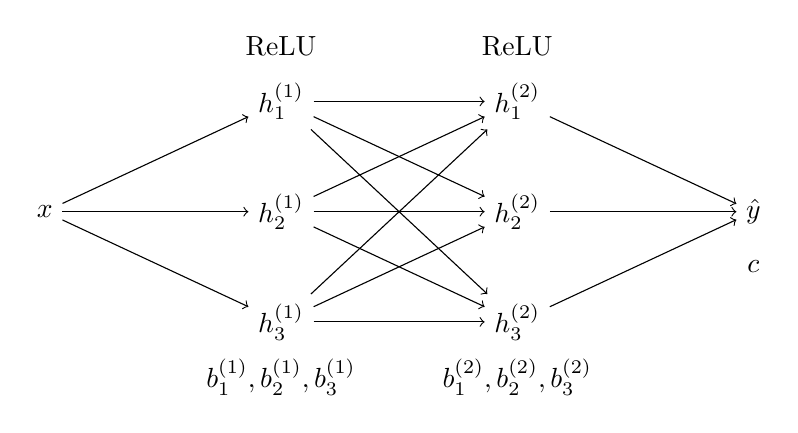
\begin{tikzpicture}
\node (x) at (0,0) {$x$};\node (y) at (9,0) {$\hat y$};
\foreach \i/\v in {1/1.4,2/0,3/-1.4} {
\node (a\i) at (3,\v) {$h^{(1)}_\i$};\node (b\i) at (6,\v) {$h^{(2)}_\i$};
\draw[->] (x)--(a\i);\draw[->] (b\i)--(y);}
\foreach \i in {1,2,3} {\foreach \j in {1,2,3} {\draw[->] (a\i)--(b\j);}}
\node at (3,2.1) {ReLU};\node at (6,2.1) {ReLU};
\node at (3,-2.1) {$b^{(1)}_1,b^{(1)}_2,b^{(1)}_3$};\node at (6,-2.1) {$b^{(2)}_1,b^{(2)}_2,b^{(2)}_3$};\node at (9,-0.7) {$c$};
\end{tikzpicture}

\end{center}

\Needspace{4\baselineskip}
\subsection{Solution 3.2 - First hidden layer}

The first-layer activations are $\operatorname{ReLU}(x)$,
$\operatorname{ReLU}(x-1)$ and $\operatorname{ReLU}(x-2)$:

\begin{center}

\begingroup
\setlength{\tabcolsep}{3pt}
\small
\begin{tabular}{@{}p{0.128\linewidth}p{0.128\linewidth}p{0.128\linewidth}p{0.128\linewidth}p{0.128\linewidth}p{0.128\linewidth}p{0.128\linewidth}@{}}
\toprule
$x_i$ & $z^{(1)}_{1,i}$ & $h^{(1)}_{1,i}$ & $z^{(1)}_{2,i}$ & $h^{(1)}_{2,i}$ & $z^{(1)}_{3,i}$ & $h^{(1)}_{3,i}$ \\
\midrule
0 & 0 & 0 & -1 & 0 & -2 & 0 \\
1 & 1 & 1 & 0 & 0 & -1 & 0 \\
2 & 2 & 2 & 1 & 1 & 0 & 0 \\
3 & 3 & 3 & 2 & 2 & 1 & 1 \\
\bottomrule
\end{tabular}
\endgroup

\end{center}

The active regions are $x>0$, $x>1$ and $x>2$. Among the training
inputs, the active sets are $\{1,2,3\}$, $\{2,3\}$ and $\{3\}$. At a
threshold the corresponding activation is still zero.

There are now three thresholds instead of two. The fitted shallow
network has thresholds 0 and 1.5; the initial network in Part I has
thresholds 0.5 and 2.5, with its second neuron active to the left of
2.5.

\Needspace{4\baselineskip}
\subsection{Solution 3.3 - Second hidden layer}

The second layer acts on the features from the first layer:

\begin{equation*}
\begin{split}
h^{(2)}_1&=\operatorname{ReLU}(h^{(1)}_1)\\
h^{(2)}_2&=\operatorname{ReLU}(h^{(1)}_1-h^{(1)}_2)\\
h^{(2)}_3&=\operatorname{ReLU}(h^{(1)}_2-h^{(1)}_3)
\end{split}
\end{equation*}

\begin{center}

\begingroup
\setlength{\tabcolsep}{3pt}
\small
\begin{tabular}{@{}p{0.128\linewidth}p{0.128\linewidth}p{0.128\linewidth}p{0.128\linewidth}p{0.128\linewidth}p{0.128\linewidth}p{0.128\linewidth}@{}}
\toprule
$x_i$ & $z^{(2)}_{1,i}$ & $h^{(2)}_{1,i}$ & $z^{(2)}_{2,i}$ & $h^{(2)}_{2,i}$ & $z^{(2)}_{3,i}$ & $h^{(2)}_{3,i}$ \\
\midrule
0 & 0 & 0 & 0 & 0 & 0 & 0 \\
1 & 1 & 1 & 1 & 1 & 0 & 0 \\
2 & 2 & 2 & 1 & 1 & 1 & 1 \\
3 & 3 & 3 & 1 & 1 & 1 & 1 \\
\bottomrule
\end{tabular}
\endgroup

\end{center}

These neurons combine already transformed features rather than receiving
the original input directly.

\Needspace{4\baselineskip}
\subsection{Solution 3.4 - Output of the deep network}

Using $\hat f_{\mathrm{deep}}=-h^{(2)}_1+4h^{(2)}_2+2h^{(2)}_3$:

\begin{center}

\begingroup
\setlength{\tabcolsep}{3pt}
\begin{tabular}{@{}p{0.234\linewidth}p{0.234\linewidth}p{0.234\linewidth}p{0.234\linewidth}@{}}
\toprule
$x_i$ & True $f(x_i)$ & Output calculation & Prediction \\
\midrule
0 & 0 & $-0+4(0)+2(0)$ & 0 \\
1 & 3 & $-1+4(1)+2(0)$ & 3 \\
2 & 4 & $-2+4(1)+2(1)$ & 4 \\
3 & 3 & $-3+4(1)+2(1)$ & 3 \\
\bottomrule
\end{tabular}
\endgroup

\end{center}

The training MSE is zero for both networks. Agreement on the four
training observations does not imply that they represent the same
function elsewhere.

\Needspace{4\baselineskip}
\subsection{Solution 3.5 - Test the network between the training points}

The first hidden layer at the new inputs is:

\begin{center}

\begingroup
\setlength{\tabcolsep}{3pt}
\small
\begin{tabular}{@{}p{0.128\linewidth}p{0.128\linewidth}p{0.128\linewidth}p{0.128\linewidth}p{0.128\linewidth}p{0.128\linewidth}p{0.128\linewidth}@{}}
\toprule
$x$ & $z^{(1)}_1$ & $h^{(1)}_1$ & $z^{(1)}_2$ & $h^{(1)}_2$ & $z^{(1)}_3$ & $h^{(1)}_3$ \\
\midrule
0.5 & 0.5 & 0.5 & -0.5 & 0 & -1.5 & 0 \\
1.25 & 1.25 & 1.25 & 0.25 & 0.25 & -0.75 & 0 \\
1.75 & 1.75 & 1.75 & 0.75 & 0.75 & -0.25 & 0 \\
2.5 & 2.5 & 2.5 & 1.5 & 1.5 & 0.5 & 0.5 \\
\bottomrule
\end{tabular}
\endgroup

\end{center}

All second-layer pre-activations are nonnegative, so each equals its
activation:

\begin{center}

\begingroup
\setlength{\tabcolsep}{3pt}
\begin{tabular}{@{}p{0.234\linewidth}p{0.234\linewidth}p{0.234\linewidth}p{0.234\linewidth}@{}}
\toprule
$x$ & $z^{(2)}_1=h^{(2)}_1$ & $z^{(2)}_2=h^{(2)}_2$ & $z^{(2)}_3=h^{(2)}_3$ \\
\midrule
0.5 & 0.5 & 0.5 & 0 \\
1.25 & 1.25 & 1 & 0.25 \\
1.75 & 1.75 & 1 & 0.75 \\
2.5 & 2.5 & 1 & 1 \\
\bottomrule
\end{tabular}
\endgroup

\end{center}

The resulting comparison is:

\begin{center}

\begingroup
\setlength{\tabcolsep}{3pt}
\begin{tabular}{@{}p{0.234\linewidth}p{0.234\linewidth}p{0.234\linewidth}p{0.234\linewidth}@{}}
\toprule
$x$ & True $f(x)$ & Shallow network & Deep network \\
\midrule
0.5 & 1.7500 & 1.5000 & 1.5000 \\
1.25 & 3.4375 & 3.7500 & 3.2500 \\
1.75 & 3.9375 & 4.2500 & 3.7500 \\
2.5 & 3.7500 & 3.5000 & 3.5000 \\
\bottomrule
\end{tabular}
\endgroup

\end{center}

At 0.5 and 2.5 the errors are equal. At 1.25 and 1.75, the deep
network\textquotesingle s absolute error is 0.1875, compared with 0.3125
for the shallow network. The models interpolate differently despite
their identical training error.

\Needspace{4\baselineskip}
\subsection{Solution 3.6 - What function has the deeper network learned?}

Evaluate the features region by region:

\begin{center}

\begingroup
\setlength{\tabcolsep}{3pt}
\begin{tabular}{@{}p{0.362\linewidth}p{0.295\linewidth}p{0.295\linewidth}@{}}
\toprule
Region & $(h^{(1)}_1,h^{(1)}_2,h^{(1)}_3)$ & $(h^{(2)}_1,h^{(2)}_2,h^{(2)}_3)$ \\
\midrule
$x<0$ & $(0,0,0)$ & $(0,0,0)$ \\
$0\leq x<1$ & $(x,0,0)$ & $(x,x,0)$ \\
$1\leq x<2$ & $(x,x-1,0)$ & $(x,1,x-1)$ \\
$x\geq2$ & $(x,x-1,x-2)$ & $(x,1,1)$ \\
\bottomrule
\end{tabular}
\endgroup

\end{center}

Substitution in $-h^{(2)}_1+4h^{(2)}_2+2h^{(2)}_3$ gives

\begin{equation*}
\hat f_{\mathrm{deep}}(x)=\begin{cases}
0 & x<0\\
-x+4x=3x & 0\leq x<1\\
-x+4+2(x-1)=x+2 & 1\leq x<2\\
-x+4+2=6-x & x\geq2
\end{cases}
\end{equation*}

The shallow network has slopes $0,3,-1$ and changes slope at 0 and 1.5.
The deep network has slopes $0,3,1,-1$ and changes slope at 0, 1 and 2.
It adds a linear region and changes the interpolation. More capacity
does not by itself guarantee better generalization.

The solid curve is the target, the dashed line the shallow network, and
the dotted line the deep network. Dots mark the training observations.

\begin{center}

\begin{tikzpicture}[x=1.45cm,y=0.48cm]
\draw[->] (-1.2,0)--(5.3,0) node[right] {$x$};
\draw[->] (0,-5.5)--(0,5.2) node[above] {$y$};
\foreach \x in {-1,1,2,3,4,5} {\draw (\x,-0.12)--(\x,0.12);\node[below] at (\x,-0.12) {\small $\x$};}
\foreach \y in {-4,-2,2,4} {\draw (-0.05,\y)--(0.05,\y);\node[left] at (-0.05,\y) {\small $\y$};}
\draw[thin,domain=-1:5,samples=81] plot (\x,{-\x*\x+4*\x});
\foreach \x/\y in {0/0,1/3,2/4,3/3} {\fill (\x,\y) circle (1.6pt);}
\draw[thick,dashed] plot coordinates {(-1,0) (0,0) (1.5,4.5) (5,1)};
\draw[very thick,dotted] plot coordinates {(-1,0) (0,0) (1,3) (2,4) (5,1)};
\end{tikzpicture}

\end{center}

\Needspace{4\baselineskip}
\section{Solutions - Conceptual questions}

\begin{enumerate}
\def\labelenumi{\arabic{enumi}.}
\tightlist
\item
  ReLU is piecewise linear. Composing it with affine transformations
  preserves a piecewise-affine form, conventionally called piecewise
  linear here.
\item
  Potential slope changes occur where ReLU pre-activations cross zero.
  In one hidden layer these positions satisfy $wx+b=0$, hence $x=-b/w$
  for $w\neq0$. Weights and biases determine the boundaries. In deeper
  layers the boundaries depend on previously constructed features. A
  zero output weight or cancellation can hide a hidden
  neuron\textquotesingle s slope change in the final output.
\item
  Output weights scale the hidden activations. Their magnitudes and
  signs determine how these contributions affect the value and slope of
  the prediction.
\item
  Two ReLU neurons can introduce two distinct thresholds and combine
  several linear regions, giving a function more flexible than a single
  straight line.
\item
  Additional neurons can add activation boundaries and learned features.
  This permits a finer approximation but also increases capacity; better
  performance on unseen data is not guaranteed.
\item
  Zero training error means agreement only at the observed inputs.
  Different functions can agree there and disagree elsewhere, so
  generalization must be assessed separately.
\end{enumerate}

\Needspace{4\baselineskip}
\section{Key concepts}

\begin{center}

\begingroup
\setlength{\tabcolsep}{3pt}
\begin{tabular}{@{}p{0.328\linewidth}p{0.638\linewidth}@{}}
\toprule
Concept & Meaning \\
\midrule
Weight / bias & Multiplicative connection / additive offset \\
Pre-activation & Affine input to an activation function \\
ReLU & $\max(0,z)$ \\
Forward pass & Compute activations and predictions \\
MSE & Average squared prediction error \\
Backpropagation & Apply the chain rule backwards to compute gradients \\
Gradient descent & Update parameters against the loss gradient \\
Piecewise-linear network & Affine behavior within each activation region \\
Generalization & Prediction quality on unseen inputs \\
\bottomrule
\end{tabular}
\endgroup

\end{center}

\end{document}
